% Fallback of erl_manuscript.tex: standard `article`, compiles with any TeX Live. Same body, abstract, back matter and references.
% Build: pdflatex erl_manuscript_article  (twice, for cross-references)
\documentclass[11pt,a4paper]{article}
\usepackage[margin=2.5cm]{geometry}
\usepackage{setspace}\onehalfspacing
\usepackage{graphicx,booktabs,amsmath,amssymb,array,url}
\usepackage[round,authoryear]{natbib}
\setcitestyle{round,aysep={},notesep={, }}
\usepackage[hidelinks]{hyperref}
\setlength{\emergencystretch}{3em}

\title{Cost-surface-driven rural road network optimization using foundation-model semantic segmentation to minimize land disturbance and structural encroachment}
\author{Pendyala Archana and Kolikipogu Ramakrishna\\[3pt]
\small Department of Information Technology, Chaitanya Bharathi Institute of Technology, Hyderabad 500075, India}
\date{}

\begin{document}
\maketitle
\begin{abstract}
\noindentExtending all-weather road access to dispersed rural hamlets is a major source of new linear infrastructure and of land disturbance, yet access routes are usually planned house by house from manually digitised building inventories. We present a framework that links satellite building detection to a cost-surface-driven shared road network and apply it to Damarakunta, an agricultural village of 18.5 square kilometres in Siddipet district, Telangana, India. Buildings were extracted from 0.6 metre imagery with a fully fine-tuned self-supervised vision-transformer segmentation network, which reached 53.8 per cent mean intersection over union (68.9 per cent mean Dice, 71.3 per cent pixel accuracy) on a public land-cover benchmark and agreed with 71.5 per cent of village candidates in an independent building layer. A ten-metre cost surface built from land cover, slope, hard terrain constraints and a penalty on building footprints drives a two-stage planner in which routes may end on existing roads or on other planned routes. For 163 residential targets and five facilities, all 168 targets were connected with no constraint violation. The shared network needs 5,069 metres of new corridor, 24.9 per cent (1,684 metres) less than independent routing, about 0.84 hectares less land under an assumed five-metre formation. The footprint penalty halves the routes crossing other dwellings, from 56 to 28, for a 7.7 per cent longer network. Across 23 simulated omission and addition runs the saving stayed between 24.9 and 26.6 per cent, but omitted buildings shortened the plan by up to 29.4 per cent and silently removed up to 38.0 per cent of households from it. Shared planning can therefore lower the land footprint of rural roads, whereas incomplete building inventories bias land-take estimates downward and should be reported as ranges. Results are model outputs for one village without field validation.

\end{abstract}
\noindent\textit{Keywords}: rural road infrastructure, remote sensing, semantic segmentation, cost-surface routing, land-use disturbance, Telangana

% Shared Letter body (Sections 1-5). Included by erl_manuscript.tex and erl_manuscript_article.tex.
% Every number is taken from DELIVERABLES_DAMARAKUNTA_STAGE_B (primary run S2_fac_C0_s25_final_x4) or from paper/erl/verify_erl_numbers.py.

\section{Introduction}
Road building is one of the largest land-use changes expected this century. Global road length is projected to grow by roughly 3.0--4.7 million km by 2050, most of it in developing economies where it opens land to clearing, fragmentation and conversion (\citealt{meijer2018global}; \citealt{laurance2014global}). Much of this growth is local. In India the Pradhan Mantri Gram Sadak Yojana (PMGSY), the national rural roads programme, connects habitations to the all-weather network (\citealt{pmgsy}), and each connection cuts a corridor through farmland and village commons. The land taken depends on a planning choice that precedes construction: how many separate corridors are built to reach the same set of houses.

Planning access to dispersed hamlets needs three inputs: where the dwellings are, what land a corridor must cross, and a rule that turns these into alignments. In practice dwellings are digitised by hand, which is slow and subjective, and each house is often treated as its own connection problem, so neighbouring houses re-trace the same corridor. Deep learning now maps buildings at continental scale (\citealt{ji2019whu}; \citealt{sirko2021openbuildings}), and vision foundation models promise better transfer to scenes with few labels (\citealt{oquab2023dinov2}; \citealt{cong2022satmae}). Least-cost-path analysis on a cost surface is the standard tool for aligning a single road or canal (\citealt{collischonn2000lcp}), and Steiner-tree heuristics describe how to connect many terminals with little shared infrastructure (\citealt{kou1981steiner}; \citealt{hwang1992steiner}). These strands are rarely joined. Detectors are scored by pixel overlap, whereas a planner consumes instances, and how detection errors propagate through a spatial analysis is seldom measured, although error propagation in geographic information systems is a long-standing problem (\citealt{heuvelink1998error}; \citealt{foody2002status}).

This Letter closes that loop for one village and makes two contributions. Contribution~1 is a measured link between satellite building detection and the road plan: controlled omission and addition of buildings are propagated through the planner to quantify their effect on corridor length, households served and exposure of dwellings. Contribution~2 is a two-stage, cost-surface-driven shared-network planner in which a route may end on an existing road or on another planned route, so that shared edges are built once; it is compared with independent routing, a length-only control and a roads-only reference. We ask how much new road footprint sharing avoids, how much a penalty on building footprints reduces structural encroachment and at what cost in length, and whether these results survive errors in the building inventory. The study is a single-village case study without field validation, and all routes are planning alternatives, not engineered alignments.

\section{Materials and methods}
\subsection{Study area and data}
Damarakunta is a rural revenue village in Markook mandal, Siddipet district, Telangana, India (about $17.707^{\circ}$N, $78.753^{\circ}$E), in the agricultural, semi-arid Deccan region. The administrative boundary, from the Telangana State Remote Sensing Application Centre (TGRAC), encloses 18.47~km$^2$ (UTM zone 44N, EPSG:32644). Settlement is dispersed: houses form small clusters separated by farmland. The TGRAC road layer has 43 features totalling 93.5~km, of which 51.7~km remain after clipping to the boundary; 44.7\% of the original length lies outside it. TGRAC records four facilities (two schools, a health sub-centre, an anganwadi child-care centre). The anganwadi was excluded because its coordinate lies 371~m from the nearest detected footprint and 126~m from the nearest independent building polygon, and two Gram Panchayat headquarters points were added, giving five facility targets.

Table~\ref{tab:data} lists the inputs. A 0.6~m, three-band mosaic (11{,}296 $\times$ 7{,}171 px) was assembled from Esri World Imagery map exports; its capture date was recorded at one sampled point only (29 April 2026). Land cover is ESA WorldCover at 10~m (\citealt{zanaga2021worldcover}). Slope is computed with a Sobel operator from an SRTM-type 30~m elevation tile (\citealt{farr2007srtm}) and resampled to 10~m, so it carries no true 10~m terrain detail. Everything is aligned to a 432 $\times$ 679 cell grid at 10~m. Cells that are water, no-data or steeper than $25^{\circ}$ are blocked; 961 slope cells and 178 land-cover cells without data are treated as invalid, not interpolated.

\begin{table}[t]
\caption{Input data and access. None of the layers was verified against ground truth.}
\label{tab:data}
\centering
\footnotesize
\begin{tabular}{@{}>{\raggedright\arraybackslash}p{3.0cm}>{\raggedright\arraybackslash}p{5.9cm}>{\raggedright\arraybackslash}p{5.3cm}@{}}
\toprule
Layer & Source and resolution & Access and status\\
\midrule
Boundary, roads, facilities & TGRAC web map services; 43 road features & Public services; licence not stated\\
High-resolution imagery & Esri World Imagery export, 0.6~m, 3 bands & Third-party; licence for derived products unresolved; not redistributed\\
Land cover & ESA WorldCover v200 (2021), 10~m; doi:10.5281/zenodo.7254221 & CC BY 4.0\\
Terrain & SRTM 1 arc-second tile n17\_e078 (30~m), doi:10.5066/F7PR7TFT & Public domain (USGS); source file name only\\
Proxy reference footprints & Google Open Buildings v3, \texttt{sites.research.google/open-buildings} & CC BY 4.0 / ODbL; agreement check only\\
Training benchmark & LoveDA, \texttt{github.com/Junjue-Wang/LoveDA} & Source domain only\\
\bottomrule
\end{tabular}
\end{table}

\subsection{Building extraction}
Building candidates are model outputs. StrongDINOv2Seg is a fully fine-tuned DINOv2 ViT-B/14 encoder (\citealt{oquab2023dinov2}) whose tokens from transformer blocks 3, 6, 9 and 12 are projected to 256 channels, fused by a feature pyramid (\citealt{lin2017fpn}), passed through an atrous spatial pyramid pooling neck (\citealt{chen2018deeplabv3plus}) and decoded by four residual up-sampling stages with auxiliary heads for deep supervision (\citealt{lee2015dsn}). The loss combines cross-entropy, soft Dice (\citealt{milletari2016vnet}) and a Sobel-weighted boundary term with weights 0.5, 0.4 and 0.1. The network was trained on LoveDA (\citealt{wang2021loveda}) with AdamW and cosine annealing over 10 epochs at 560~px, and the epoch-4 checkpoint with the best validation score was applied to the mosaic in $560\times560$~px tiles (stride 420~px). The class map was converted to instances by a distance-transform procedure: adjacent roofs are separated only where the saddle between them is narrower than 0.65 times the inscribed radius of the smaller piece, and polygons much larger than a typical roof are flagged as unresolved merges instead of being cut. This gave 278 candidate polygons, 165 inside the boundary, of which 163 were retained as house targets: 71 plausible, 32 needing review and 62 unresolved merges. The representative point of each polygon is a routing target with weight one. Figure~\ref{fig:workflow} summarises the workflow.

No pixel-level reference exists for Damarakunta, so two evaluations are kept apart: source-domain validation on LoveDA, and a proxy agreement check of the village candidates against Open Buildings (a candidate agrees if an Open Buildings polygon lies within 30~m). Agreement is not accuracy, and neither layer is treated as truth.

\begin{figure}[t]
\centering
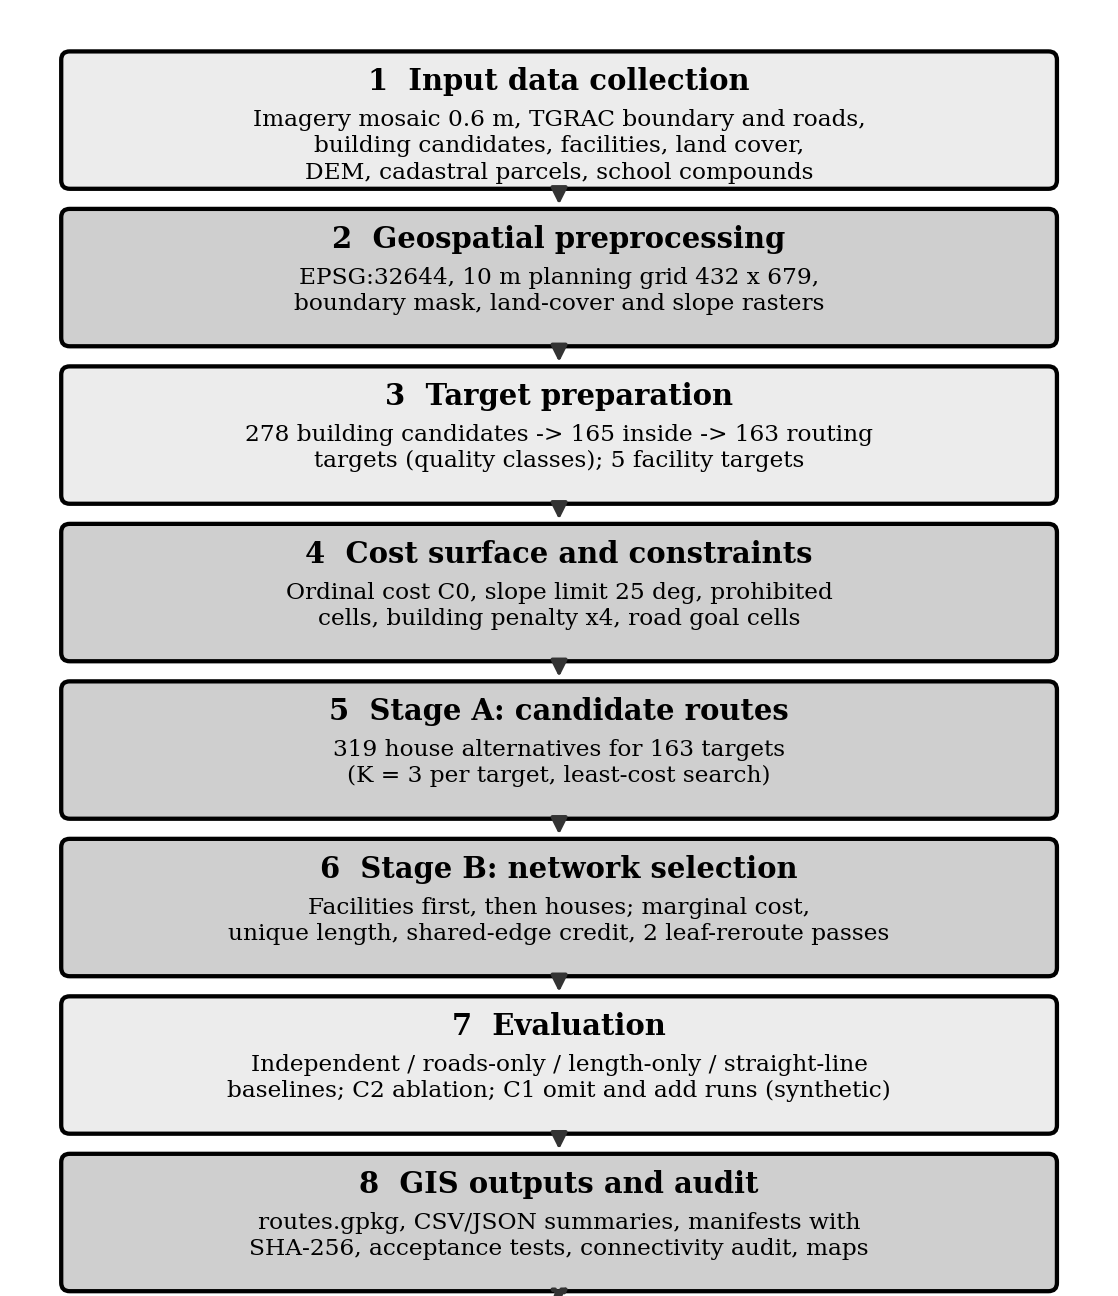
\includegraphics[height=0.62\textheight]{figures/fig1_architecture_phase1.png}
\caption{Framework from input data to GIS outputs. Dark boxes were implemented and run; light boxes were implemented but depend on unverified inputs or synthetic evidence (building candidates, evaluation experiments).}
\label{fig:workflow}
\end{figure}

\subsection{Cost surface}
Let $\mathcal{B}$ be the blocked cells (water, no-data, slope above $25^{\circ}$) and $\mathcal{P}$ the cells that intersect a candidate footprint. The planning graph has the unblocked cells as nodes and 8-neighbour edges. The ordinal cost of a cell $x$ with land-cover class $\ell(x)$ and slope $s(x)$ in degrees is
\begin{equation}
c(x)=\Bigl[c_{\mathrm{lc}}\bigl(\ell(x)\bigr)+w_s\,\frac{\min\{s(x),s_{\max}\}}{s_{\max}}\Bigr]\,m(x),\qquad m(x)=\begin{cases}\mu & x\in\mathcal{P}\\ 1 & \text{otherwise,}\end{cases}
\label{eq:cell}
\end{equation}
with $w_s=4$, $s_{\max}=10^{\circ}$ and base costs $c_{\mathrm{lc}}$ of 8 for tree cover, 6 for cropland, 5 for shrubland, 4 for bare or sparse vegetation, 3 for grassland and 2 for built-up land. Costs therefore range from 2.09 to 12.0 before the footprint multiplier, and the primary penalty is $\mu=4$. The weight of an edge between neighbouring cells $i$ and $j$ is the mean of the end-cell costs times the step length $d_{ij}$,
\begin{equation}
w_{ij}=d_{ij}\,\frac{c(i)+c(j)}{2}.
\label{eq:edge}
\end{equation}
Costs are ordinal planning units, not currency. Around the health sub-centre, whose point lies on the edge of its own footprint, the penalty is lifted within a 20~m disc so that the route is not forced to detour around its own building; crossing statistics are always computed on the original footprints.

\subsection{Shared-network planner}
Stage~A computes, for every target, a least-cost path to the road cells with a Dijkstra-type search (\citealt{dijkstra1959note}; \citealt{hart1968astar}) and up to two further alternatives obtained by inflating costs in a 20~m corridor around earlier paths (319 alternatives for 163 houses). Stage~B selects greedily the pair of target and alternative with the highest weight per marginal cost,
\begin{equation}
\Delta L_{\mathrm{cost}}(\pi\mid S)=\sum_{e\in\pi\setminus E_S}w_e,
\label{eq:marginal}
\end{equation}
where $E_S$ is the set of edges already selected, so that built edges are free and a route may end on another route. This is the shortest-path heuristic for Steiner trees (\citealt{kou1981steiner}; \citealt{mehlhorn1988steiner}) applied to a penalised, land-cover-weighted graph with the road network as a free sub-tree; it has no optimality guarantee. Two passes of leaf re-routing follow, and facilities are planned before houses. The plan is compared with straight lines, independent least-cost routes, a length-only control (shortest distance under the same constraints) and a roads-only shared reference. With $L(\cdot)$ the unique edge length, the saving is
\begin{equation}
\rho=100\,\frac{L_{\mathrm{indep}}-L_{\mathrm{plan}}}{L_{\mathrm{indep}}},
\label{eq:saving}
\end{equation}
and the land take of a network of unique length $L$ and assumed formation width $b$ is $A=bL$, with $b=5$~m an assumption of this study.

\subsection{Perturbation analysis}
Let $T$ be the target set and $M\subset T$ an omitted set standing for false negatives. The planner is re-run on $T\setminus M$ with the footprints of $M$ also removed from the penalty layer, because a missed detection is absent from both the target list and the obstacle layer. We report households left without a route, the change in unique length and the length per routed target, which is the comparable quantity because absolute length shrinks mechanically when fewer targets are connected. The scenarios are random omission of 10\% and 20\% of targets and random addition of 10\% and 20\% synthetic targets (five draws each, 20 runs), omission of the smallest 10\% and 25\% of targets by footprint area, and omission of all 62 unresolved merges (three deterministic runs). The 23 perturbed runs are synthetic and are not measured detection errors.

\section{Results}
\subsection{Segmentation and detection agreement}
On the 1{,}669-image LoveDA validation split (560~px, seven scored classes) the checkpoint reached 53.8\% mean intersection over union (mIoU), 68.9\% mean Dice and 71.3\% pixel accuracy (table~\ref{tab:seg}); these are source-domain figures, not accuracy in Damarakunta. For the building class the intersection over union is 54.0\%, with 62.1\% precision and 80.6\% recall. Of the 165 in-boundary candidates, 118 (71.5\%) agree with Open Buildings, ranging from 43.8\% for the review class to 85.5\% for unresolved merges; high agreement of merged blobs says nothing about whether a blob holds one house or several. Open Buildings lists 1{,}537 polygons in the boundary, 1{,}186 of them without a candidate, so the 163 targets are a conservative planning set, not a house count. All five facilities lie within 8.5~m of a detected footprint and within 8.7~m of an independent polygon.

\begin{table}[t]
\caption{Detection evaluation. Top: LoveDA validation split, in per cent. Bottom: agreement of the 165 Damarakunta candidates with Open Buildings v3 (a proxy, not accuracy).}
\label{tab:seg}
\centering
\small
\begin{tabular}{@{}lrrrrr@{}}
\toprule
\multicolumn{6}{@{}l}{\textit{LoveDA validation split}}\\
 & mIoU & Dice & Pixel acc. & Precision & Recall\\
\midrule
StrongDINOv2Seg (all classes) & 53.8 & 68.9 & 71.3 & 72.4 & 66.9\\
\quad building class & 54.0 & 70.1 & --- & 62.1 & 80.6\\
\midrule
\multicolumn{6}{@{}l}{\textit{Damarakunta candidates against Open Buildings v3}}\\
Class & Candidates & Agree & Disagree & \multicolumn{2}{c}{Agreement (\%)}\\
\midrule
All & 165 & 118 & 47 & \multicolumn{2}{c}{71.5}\\
Plausible & 71 & 51 & 20 & \multicolumn{2}{c}{71.8}\\
Review & 32 & 14 & 18 & \multicolumn{2}{c}{43.8}\\
Unresolved merge & 62 & 53 & 9 & \multicolumn{2}{c}{85.5}\\
\bottomrule
\end{tabular}
\end{table}

\subsection{Shared versus independent road network}
Independent least-cost routes for the 163 houses total 10{,}045~m, but neighbouring houses re-trace the same corridors, so the unique built length is 6{,}753~m (table~\ref{tab:routing}, figure~\ref{fig:lengths}). The two-stage plan needs 5{,}069~m, a saving of 1{,}684~m (24.9\%). All 163 houses and five facilities are connected (168 of 168 verified by the planner) with no hard-constraint violation, no cycle and no route crossing another without a shared cell. A length-only control is longer in unique length than independent least-cost routing (6{,}980~m) and crosses other footprints on 64 routes, so the cost surface, not shortness alone, produces the gain. The roads-only shared reference (5{,}229~m) is 160~m longer than the two-stage plan, so ending routes on other routes adds a modest further saving of 2.3 percentage points. Extra alternatives per target change nothing in this village and leaf re-routing contributes 10.3~m (0.2\%), so the saving comes mainly from sharing itself. One house attaches to a road fragment that the raster treats as a separate component, a boundary-truncation artefact of the clipped domain: on the TGRAC road lines all 168 targets connect to the main network.

\begin{table}[t]
\caption{Routing for 163 houses ($\mu=4$ unless stated). Unique length counts shared edges once; crossing routes pass through another house footprint; $\rho$ is the saving in unique length against independent least-cost routes planned under the same penalty.}
\label{tab:routing}
\centering
\footnotesize\setlength{\tabcolsep}{4pt}
\begin{tabular}{@{}>{\raggedright\arraybackslash}p{4.3cm}rrrrr@{}}
\toprule
Strategy & Total (m) & Unique (m) & $\rho$ (\%) & Crossing routes & In footprints (m)\\
\midrule
Straight line (2 targets infeasible) & 8{,}092.3 & --- & --- & 60 & 1{,}453.2\\
Independent least-cost routes & 10{,}045.4 & 6{,}753.1 & 0.0 & 46 & 328.3\\
Length-only control & 9{,}166.3 & 6{,}979.8 & $-3.4$ & 64 & 1{,}615.8\\
Roads-only shared reference & 5{,}229.3 & 5{,}229.3 & 22.6 & 29 & 216.1\\
\textbf{Two-stage plan (proposed)} & \textbf{5{,}069.0} & \textbf{5{,}069.0} & \textbf{24.9} & \textbf{28} & \textbf{209.1}\\
\midrule
\multicolumn{6}{@{}l}{\textit{No footprint penalty ($\mu=1$)}}\\
Independent least-cost routes & 9{,}595.9 & 6{,}921.3 & 0.0 & 63 & 1{,}423.1\\
Two-stage plan & 4{,}705.5 & 4{,}705.4 & 32.0 & 56 & 660.1\\
\midrule
\multicolumn{6}{@{}l}{\textit{Footprints buffered by 7.1~m, two-stage plan}}\\
Penalty $\mu=20$ & --- & 6{,}238.1 & 18.5 & 19 & 147.9\\
Penalty $\mu=100$ & --- & 6{,}190.3 & 18.9 & 19 & 144.8\\
\bottomrule
\end{tabular}
\end{table}

\begin{figure}[t]
\centering
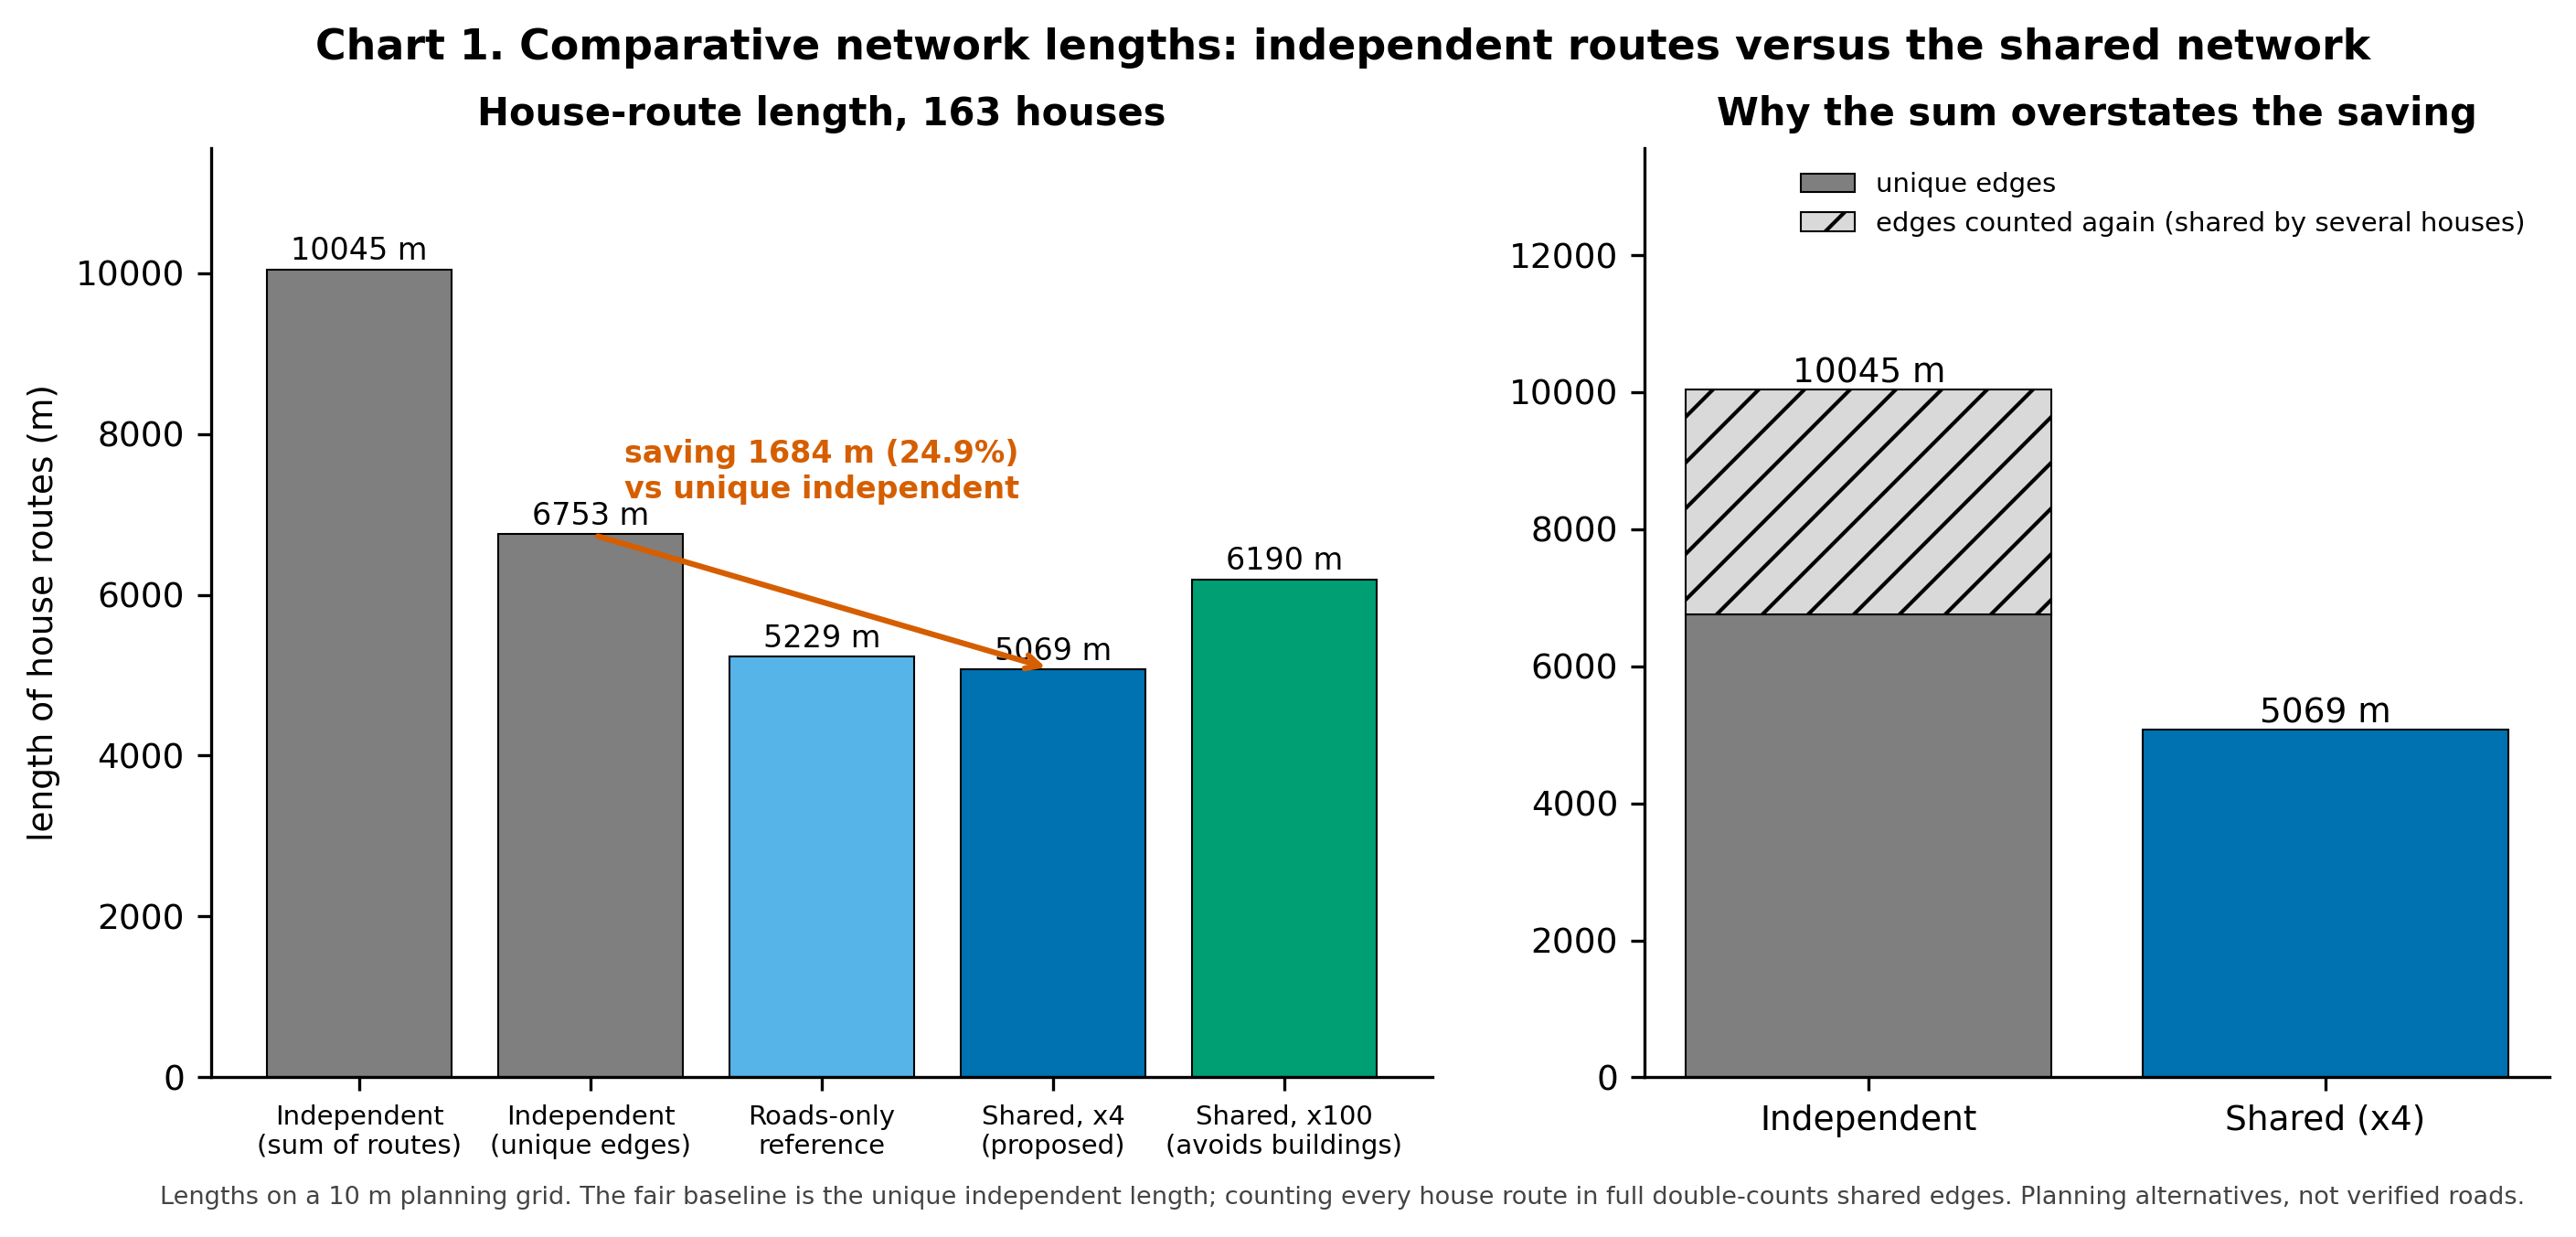
\includegraphics[width=\textwidth]{figures/chart1_network_lengths.png}
\caption{House-route lengths for independent routing and shared networks. The sum of independent routes (10{,}045~m) double-counts edges used by several houses, so the fair baseline is the unique independent length (6{,}753~m); the shared plan (5{,}069~m) saves 1{,}684~m (24.9\%).}
\label{fig:lengths}
\end{figure}

\subsection{Structural encroachment and the footprint penalty}
The footprint penalty trades corridor length against encroachment on dwellings (figure~\ref{fig:avoid}). With no penalty the shared plan is shortest (4{,}705~m) but 56 routes pass through other houses (660~m inside footprints). With $\mu=4$ the plan is 364~m (7.7\%) longer and the number of routes crossing another footprint halves to 28 (209~m inside footprints). Against independent routing under the same penalty, the shared plan also has fewer crossing routes (28 against 46). Buffering footprints by 7.1~m with penalties of 20 to 1000 lowers crossings to 19 routes (145--148~m) but adds 1.1--1.2~km of corridor and erodes the saving to 18.5--19.2\%; the effect saturates by $\mu=20$. Hard blocking was infeasible because every house point lies inside its own blocked cell, and 16 of the 19 remaining crossings occur within the first 20~m of a route, where it leaves its own cluster of touching buildings. This is a property of the detections and the 10~m grid, not of the cost function.

\begin{figure}[t]
\centering
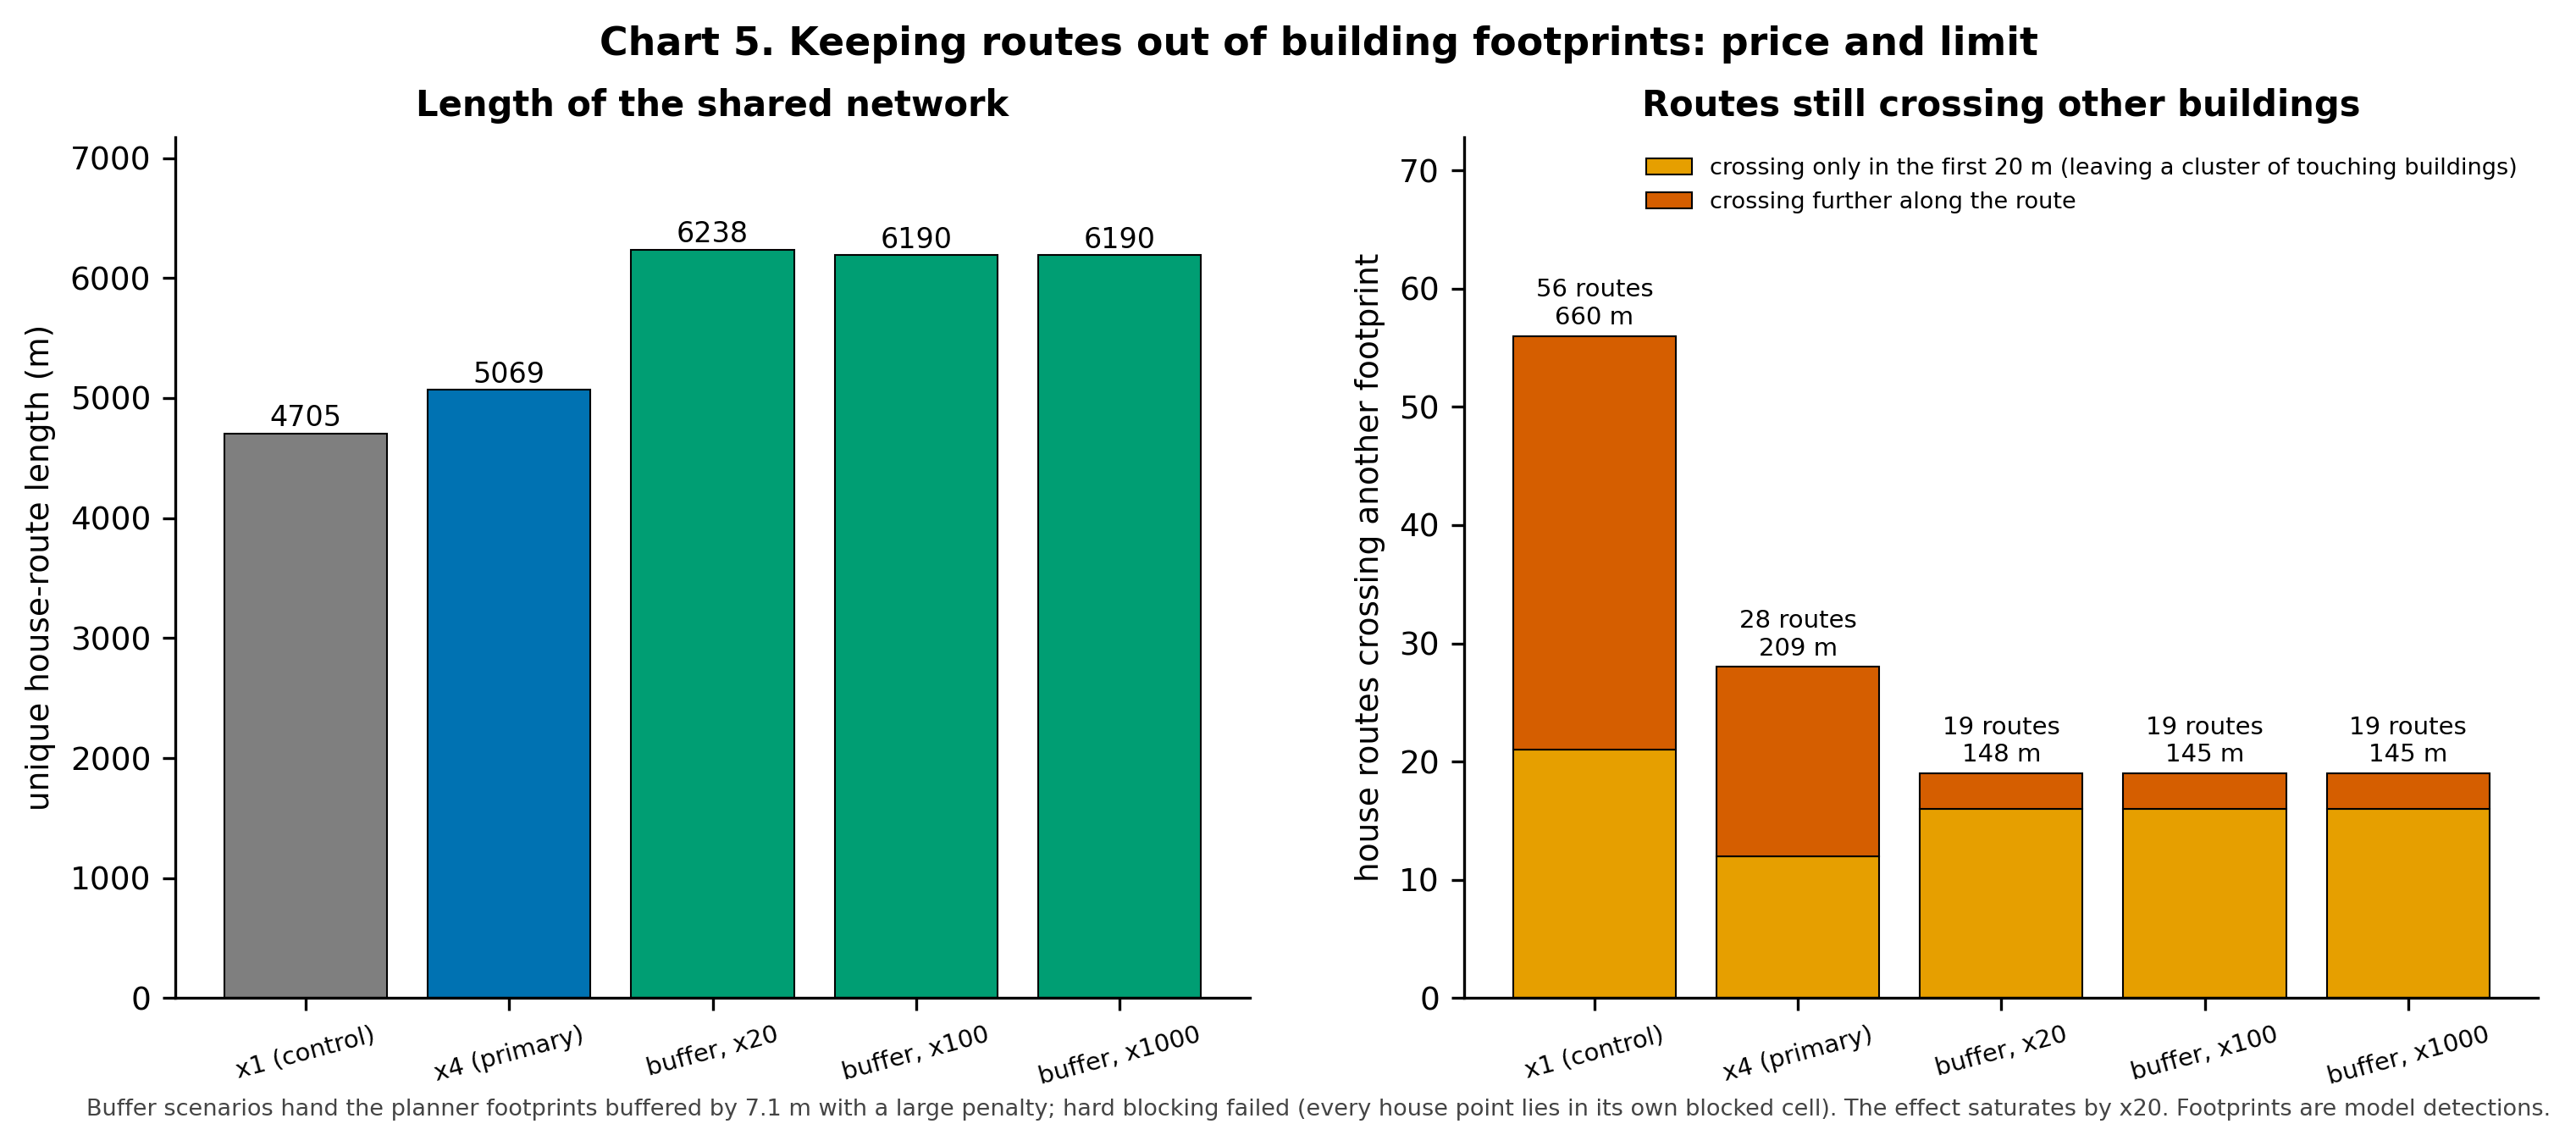
\includegraphics[width=\textwidth]{figures/chart5_obstacle_avoidance_tradeoff.png}
\caption{Building avoidance. Left: unique network length for no penalty ($\mu=1$), the primary penalty ($\mu=4$) and buffered footprints with penalties of 20, 100 and 1000. Right: routes still crossing another footprint, split into crossings confined to the first 20~m and crossings further along the route.}
\label{fig:avoid}
\end{figure}

\subsection{Robustness to detection errors}
Table~\ref{tab:omission} and figure~\ref{fig:omission} summarise the 23 perturbed runs against the 5{,}069~m baseline. Every placed target was routed in every run, and the saving $\rho$ against independent routing stays between 24.9\% and 26.6\% across all scenarios, so the benefit of sharing is robust. Absolute length is not: omitting 10\% and 20\% of buildings at random shortens the plan by 7.6\% and 16.9\% and leaves 16 and 33 households without any route, and omitting all unresolved merges shortens it by 29.4\% and leaves 62 households (38.0\%) unserved. Length per routed target is stable under random omission (31.9~m and 32.4~m against 31.1~m) but rises 14\% when merged blobs are removed (35.4~m), because the remaining targets are peripheral. Random additions of 10\% and 20\% lengthen the plan by 8.6\% and 15.8\%.

\begin{table}[t]
\caption{Effect of simulated omissions and additions on the shared network (baseline 5{,}069.0~m, 163 routed). Random scenarios are means of five draws; the other three omission scenarios are single runs. $\rho$: saving against independent routing.}
\label{tab:omission}
\centering
\small
\begin{tabular}{@{}lrrrrrr@{}}
\toprule
Scenario & Routed & Unserved & Length (m) & Change (\%) & Per target (m) & $\rho$ (\%)\\
\midrule
Baseline & 163 & 0 & 5{,}069.0 & 0.0 & 31.1 & 24.9\\
Omit 10\% (random) & 147.0 & 16 & 4{,}684.4 & $-7.6$ & 31.9 & 25.1\\
Omit 20\% (random) & 130.0 & 33 & 4{,}211.5 & $-16.9$ & 32.4 & 24.9\\
Omit smallest 10\% & 146 & 17 & 4{,}648.6 & $-8.3$ & 31.8 & 24.9\\
Omit smallest 25\% & 122 & 41 & 3{,}798.3 & $-25.1$ & 31.1 & 25.6\\
Omit unresolved merges & 101 & 62 & 3{,}579.0 & $-29.4$ & 35.4 & 26.6\\
Add 10\% (random) & 177.4 & --- & 5{,}502.4 & $+8.6$ & 31.0 & 25.6\\
Add 20\% (random) & 190.6 & --- & 5{,}868.3 & $+15.8$ & 30.8 & 25.4\\
\bottomrule
\end{tabular}
\end{table}

\begin{figure}[t]
\centering
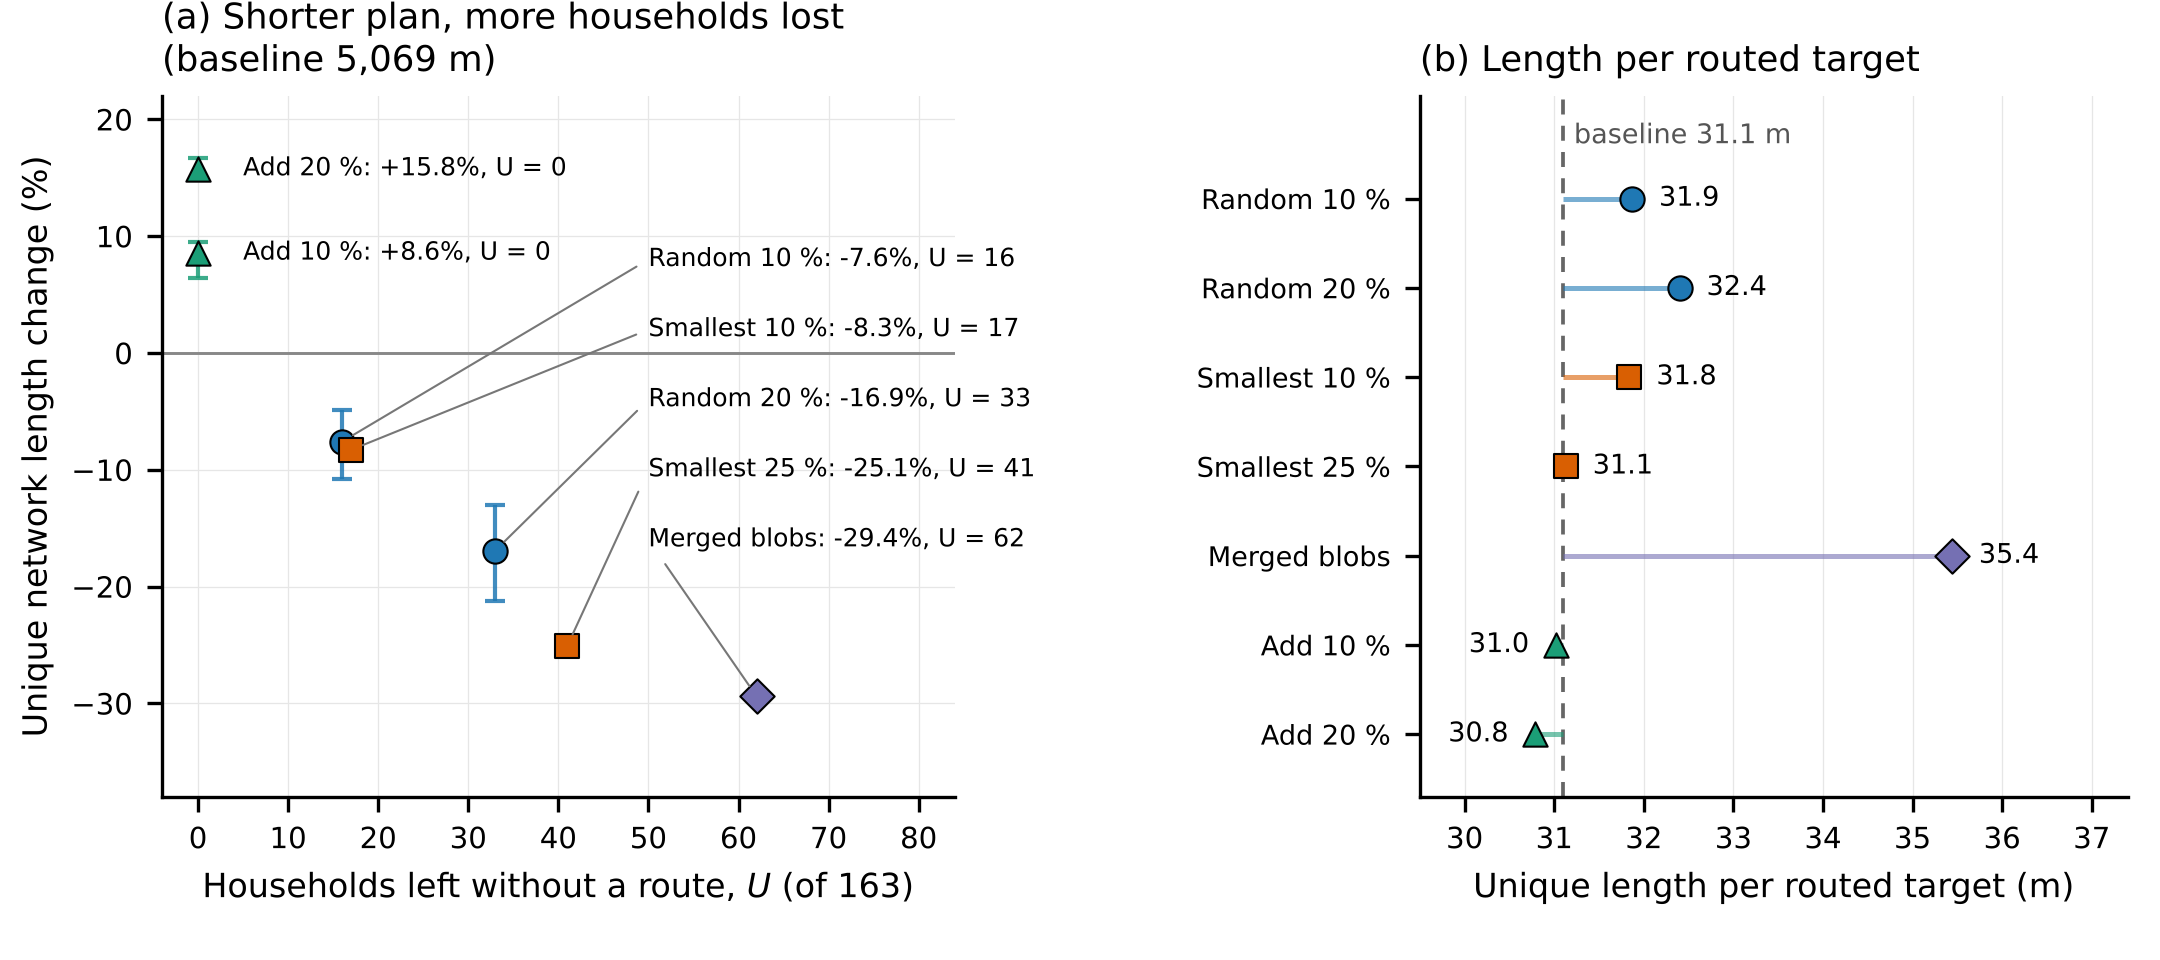
\includegraphics[width=\textwidth]{figures/fig4_omission.png}
\caption{Omission sensitivity (163 baseline targets, 5{,}069~m; random scenarios show five draws with minimum--maximum bars). Left: change in unique length against households left without a route; every omission shortens the plan while losing households, whereas additions lengthen it. Right: unique length per routed target.}
\label{fig:omission}
\end{figure}

\section{Discussion}
\subsection{Land take and construction cost}
Sharing corridors reduces new road footprint for the same households. Under an assumed 5~m formation width, the 5{,}069~m shared network occupies about 2.53~ha against 3.38~ha for the unique independent network, a saving of 0.84~ha of mostly agricultural land. The footprint penalty moves the other way: keeping routes out of dwellings costs length, and the buffered variant adds 1.1--1.2~km, roughly 0.6~ha at the same width, to reduce crossing routes from 28 to 19. A planner therefore needs the length--encroachment curve (figure~\ref{fig:avoid}), not a single number, and the primary penalty of 4 halves crossings for 7.7\% more length, whereas removing nine further crossing routes by buffering costs 1.1--1.2~km more (table~\ref{tab:routing}).

At the programme-based rate of Rs~75~lakh~km$^{-1}$ supplied by the project owner, which was not checked against a PMGSY document or a State Schedule of Rates, the 1{,}684~m saved corresponds to about Rs~126~lakh (Rs~101--152~lakh for rates of Rs~60--90~lakh~km$^{-1}$). The estimate is illustrative: the routes are mostly short house lanes of about 31~m per house for which a habitation-connectivity rate may not apply, and the cost surface does not encode Indian Roads Congress or PMGSY technical specifications such as curvature, width, drainage or gradient beyond the $25^{\circ}$ block. Comparing the baselines on unique length matters: subtracting the shared network from the double-counted total would give 4{,}976~m, three times the real saving.

\subsection{Why detection quality matters for environmental planning}
Pixel scores are area-weighted over classes, whereas a planner counts instances. A detector that misses the smallest quarter of buildings by count can lose only a small share of building pixels yet removes a quarter of the households from the plan; one that merges adjacent roofs can score a high overlap yet removes 38.0\% of the targets in one stroke (table~\ref{tab:omission}). An inventory missing 20\% of buildings would also suggest 16.9\% less corridor, and hence less land take, than the full set requires, so incomplete inventories bias land-take estimates downward. Detection studies intended for infrastructure use should therefore report instance-level recall and the households a downstream plan would leave unserved alongside overlap scores.

\subsection{Limitations and scalability}
The study covers one village and the perturbations are synthetic. The candidate layer has no surveyed reference, and the LoveDA scores come from the epoch-4 checkpoint whose metadata were recovered from the training notebook. The planner is greedy and not globally optimal, shared-edge credit counts only identical grid edges, and costs are ordinal. Slope derives from a 30~m elevation model of recorded file name but unrecorded provenance, the road layer is of unverified completeness, imagery capture dates are known at one point only, and the licence for derived products of the Esri imagery has not been cleared, so imagery is not shown or redistributed. Seasonal occlusion by canopy, shadow and crop cover is not modelled, and the area of cropland or trees crossed by the planned routes was not quantified, which would be the natural next step for agricultural land-conservation questions. Whether the 24.9\% saving transfers to other settlement morphologies, for example compact nucleated villages where sharing is already implicit or highly scattered hamlets where it is rarer, is untested; the saving is expected to depend on how clustered the houses are, and it should be measured on villages with hand-labelled buildings before any programme-level claim.

\section{Conclusions}
A pipeline from satellite imagery to a shared rural access network connected all 163 houses and five facilities of Damarakunta with 5{,}069~m of new corridor, 24.9\% (1{,}684~m) less than independent routing, and a building-footprint penalty halved the number of routes crossing other dwellings, from 56 to 28, for a 7.7\% longer network. The relative saving held between 24.9\% and 26.6\% across 23 synthetic perturbations, but absolute length and household coverage did not: omitted buildings shorten the plan and silently remove households from it. Rural road planning that relies on automatically extracted buildings should therefore treat corridor length and land take as ranges, report instance-level recall, and validate detections on a labelled subset before use. Field validation and transfer to other villages remain open.

% Shared ERL back matter. \roles and \suppdata are IOP macros; \providecommand keeps this file compiling with plain article.
\providecommand{\roles}[1]{#1}
\providecommand{\suppdata}[2]{#2 (\url{#1})}

\section*{Acknowledgments}
The authors thank the Telangana State Remote Sensing Application Centre (TGRAC) for the village boundary, road and facility layers, and the providers of the open datasets used: ESA WorldCover, Google Open Buildings, SRTM (USGS) and LoveDA. The work was carried out as part of the M.Tech dissertation of the first author at the Department of Information Technology, Chaitanya Bharathi Institute of Technology, Hyderabad.

\section*{Funding}
This research received no specific grant from any funding agency in the public, commercial or not-for-profit sectors.

\section*{Author contributions}
\roles{Pendyala Archana: Conceptualization, Methodology, Software, Validation, Writing -- original draft. Dr.~Kolikipogu Ramakrishna: Supervision, Project administration, Writing -- review \& editing.}

\section*{Conflict of interest}
The authors declare no competing interests.

\section*{Data availability statement}
\suppdata{https://github.com/Archana519/Telangana-Rural-Project}{The code (planner, analysis and figure scripts), the derived result tables of the routing, ablation and omission runs, and the building-candidate and planning layers derived from TGRAC data are openly available in the project repository} (folders \texttt{DELIVERABLES\_DAMARAKUNTA\_STAGE\_B}, \texttt{paper/erl} and \texttt{Manuscript\_ERL\_Phase1}); the repository is the access point until an archive with a persistent identifier is deposited. The LoveDA epoch-4 confusion matrix behind the reported segmentation scores is in \texttt{paper/erl/supplementary}. Public input datasets are available from their providers: ESA WorldCover v200 (\url{https://doi.org/10.5281/zenodo.7254221}), SRTM 1 arc-second (\url{https://doi.org/10.5066/F7PR7TFT}), Google Open Buildings (\url{https://sites.research.google/open-buildings/}) and LoveDA (\url{https://github.com/Junjue-Wang/LoveDA}). The 0.6~m Esri World Imagery mosaic is third-party data and is not redistributed because the licence for derived products has not been cleared. The TGRAC layers are third-party data whose licence terms are not stated, so the derived planning layers are shared for review subject to the data holder's terms. The geometry of the planned routes of the primary run is not archived.

\begin{thebibliography}{99}
\providecommand{\url}[1]{\texttt{#1}}
\bibitem[{Chen {\it et al}(2018)}]{chen2018deeplabv3plus} Chen L C, Zhu Y, Papandreou G, Schroff F and Adam H 2018 Encoder-Decoder with Atrous Separable Convolution for Semantic Image Segmentation Proceedings of the European Conference on Computer Vision (ECCV) pp 833--851

\bibitem[{Collischonn and Pilar(2000)}]{collischonn2000lcp} Collischonn W and Pilar J V 2000 A Direction Dependent Least-Cost-Path Algorithm for Roads and Canals {\it Int. J. Geogr. Inf. Sci.} {\bf 14} 397--406 doi:10.1080/13658810050024304

\bibitem[{Cong {\it et al}(2022)}]{cong2022satmae} Cong Y, Khanna S, Meng C, Liu P, Rozi E, He Y, Burke M, Lobell D and Ermon S 2022 {SatMAE}: Pre-training Transformers for Temporal and Multi-Spectral Satellite Imagery Advances in Neural Information Processing Systems vol 35

\bibitem[{Dijkstra(1959)}]{dijkstra1959note} Dijkstra E W 1959 A Note on Two Problems in Connexion with Graphs {\it Numer. Math.} {\bf 1} 269--271 doi:10.1007/BF01386390

\bibitem[{Farr {\it et al}(2007)}]{farr2007srtm} Farr T G, Rosen P A, Caro E, Crippen R, Duren R, Hensley S, Kobrick M, Paller M, Rodriguez E, Roth L, Seal D, Shaffer S, Shimada J, Umland J, Werner M, Oskin M, Burbank D and Alsdorf D 2007 The Shuttle Radar Topography Mission {\it Rev. Geophys.} {\bf 45} RG2004 doi:10.1029/2005RG000183

\bibitem[{Foody(2002)}]{foody2002status} Foody G M 2002 Status of Land Cover Classification Accuracy Assessment {\it Remote Sens. Environ.} {\bf 80} 185--201 doi:10.1016/S0034-4257(01)00295-4

\bibitem[{Hart {\it et al}(1968)}]{hart1968astar} Hart P E, Nilsson N J and Raphael B 1968 A Formal Basis for the Heuristic Determination of Minimum Cost Paths {\it IEEE Trans. Syst. Sci. Cybern.} {\bf 4} 100--107 doi:10.1109/TSSC.1968.300136

\bibitem[{Heuvelink(1998)}]{heuvelink1998error} Heuvelink G B M 1998 Error Propagation in Environmental Modelling with {GIS} Taylor \& Francis, London

\bibitem[{Hwang {\it et al}(1992)}]{hwang1992steiner} Hwang F K, Richards D S and Winter P 1992 The {Steiner} Tree Problem North-Holland, Amsterdam

\bibitem[{Ji {\it et al}(2019)}]{ji2019whu} Ji S, Wei S and Lu M 2019 Fully Convolutional Networks for Multisource Building Extraction From an Open Aerial and Satellite Imagery Data Set {\it IEEE Trans. Geosci. Remote Sens.} {\bf 57} 574--586 doi:10.1109/TGRS.2018.2858817

\bibitem[{Kou {\it et al}(1981)}]{kou1981steiner} Kou L, Markowsky G and Berman L 1981 A Fast Algorithm for {Steiner} Trees {\it Acta Inform.} {\bf 15} 141--145 doi:10.1007/BF00288961

\bibitem[{Laurance {\it et al}(2014)}]{laurance2014global} Laurance W F, Clements G R, Sloan S, O'Connell C S, Mueller N D, Goosem M, Venter O, Edwards D P, Phalan B, Balmford A, Van Der Ree R and Arrea I B 2014 A Global Strategy for Road Building {\it Nature} {\bf 513} 229--234 doi:10.1038/nature13717

\bibitem[{Lee {\it et al}(2015)}]{lee2015dsn} Lee C Y, Xie S, Gallagher P, Zhang Z and Tu Z 2015 Deeply-Supervised Nets Proceedings of the 18th International Conference on Artificial Intelligence and Statistics (AISTATS) vol 38 pp 562--570

\bibitem[{Lin {\it et al}(2017)}]{lin2017fpn} Lin T Y, Doll{\'a}r P, Girshick R, He K, Hariharan B and Belongie S 2017 Feature Pyramid Networks for Object Detection Proceedings of the IEEE Conference on Computer Vision and Pattern Recognition (CVPR) pp 2117--2125

\bibitem[{Mehlhorn(1988)}]{mehlhorn1988steiner} Mehlhorn K 1988 A Faster Approximation Algorithm for the {Steiner} Problem in Graphs {\it Inf. Process. Lett.} {\bf 27} 125--128 doi:10.1016/0020-0190(88)90066-X

\bibitem[{Meijer {\it et al}(2018)}]{meijer2018global} Meijer J R, Huijbregts M A J, Schotten K C G J and Schipper A M 2018 Global Patterns of Current and Future Road Infrastructure {\it Environ. Res. Lett.} {\bf 13} 064006 doi:10.1088/1748-9326/aabd42

\bibitem[{Milletari {\it et al}(2016)}]{milletari2016vnet} Milletari F, Navab N and Ahmadi S A 2016 {V-Net}: Fully Convolutional Neural Networks for Volumetric Medical Image Segmentation Fourth International Conference on 3D Vision (3DV) pp 565--571

\bibitem[{Ministry of Rural Development, Government of India(2026)}]{pmgsy} Ministry of Rural Development, Government of India 2026 Pradhan Mantri Gram Sadak Yojana ({PMGSY}) \url{https://pmgsy.nic.in} Accessed: Nov. 14, 2026

\bibitem[{Oquab {\it et al}(2024)}]{oquab2023dinov2} Oquab M, Darcet T, Moutakanni T, Vo H, Szafraniec M, Khalidov V, Fernandez P, Haziza D, Massa F, El-Nouby A, Assran M, Ballas N, Galuba W, Howes R, Huang P Y, Li S W, Misra I, Rabbat M, Sharma V, Synnaeve G, Xu H, Jegou H, Mairal J, Labatut P, Joulin A and Bojanowski P 2024 {DINOv2}: Learning Robust Visual Features without Supervision {\it Trans. Mach. Learn. Res.} (arXiv:2304.07193)

\bibitem[{Sirko {\it et al}(2021)}]{sirko2021openbuildings} Sirko W, Kashubin S, Ritter M, Annkah A, Bouchareb Y S E, Dauphin Y, Keysers D, Neumann M, Cisse M and Quinn J 2021 Continental-Scale Building Detection from High Resolution Satellite Imagery arXiv:2107.12283

\bibitem[{Wang {\it et al}(2021)}]{wang2021loveda} Wang J, Zheng Z, Ma A, Lu X and Zhong Y 2021 {LoveDA}: A Remote Sensing Land-Cover Dataset for Domain Adaptive Semantic Segmentation Advances in Neural Information Processing Systems, Datasets and Benchmarks Track (arXiv:2110.08733)

\bibitem[{Zanaga {\it et al}(2022)}]{zanaga2021worldcover} Zanaga D, Van De Kerchove R, De Keersmaecker W, Souverijns N, Brockmann C, Quast R, Wevers J, Grosu A, Paccini A, Vergnaud S, Cartus O, Santoro M, Fritz S, Georgieva I, Lesiv M, Carter S, Herold M, Li L, Tsendbazar N E, Ramoino F and Arino O 2022 {ESA WorldCover} 10~m 2021 v200 Zenodo doi:10.5281/zenodo.7254221

\end{thebibliography}
\end{document}
